\documentclass{standalone}

%~~~~ SPACING
\usepackage{setspace}

%~~~~ FONT AND GRAMMAR CHECKER
\usepackage[T1]{fontenc}
\usepackage[utf8]{inputenc}
\usepackage[english]{babel}

%~~~~ TEXT COLOR
\usepackage[usenames,dvipsnames,svgnames,table]{xcolor}

%~~~~ HYPERLINK
\usepackage{url}
\usepackage[colorlinks=true,
			citecolor=green!50!black, 
			linkcolor=cyan!50!blue]{hyperref}

%~~~~ MATH
\usepackage{amsmath}
\usepackage{mathtools}
\usepackage{xfrac}
\usepackage{cancel}
\usepackage{mathrsfs} % per fare la L di L-circuit $\mathscr{L}$
\usepackage{dsfont} % per le matrici dello ssm

%~~~~ FIGURES & TABLES
\usepackage{graphicx}
\usepackage{multirow, adjustbox}
\usepackage{subcaption}

% ~~~~ TIKZ
\usepackage{tikz, circuitikz}
\usetikzlibrary{shapes,
				arrows,
				calc,
				patterns,
				decorations.pathmorphing,
				decorations.markings}

\usepackage{3dplot} %requires 3dplot.sty to be in same directory, or in your LaTeX installation			

\begin{document}

% \input{drawings/bonnie}

% \input{drawings/sarsa}

% 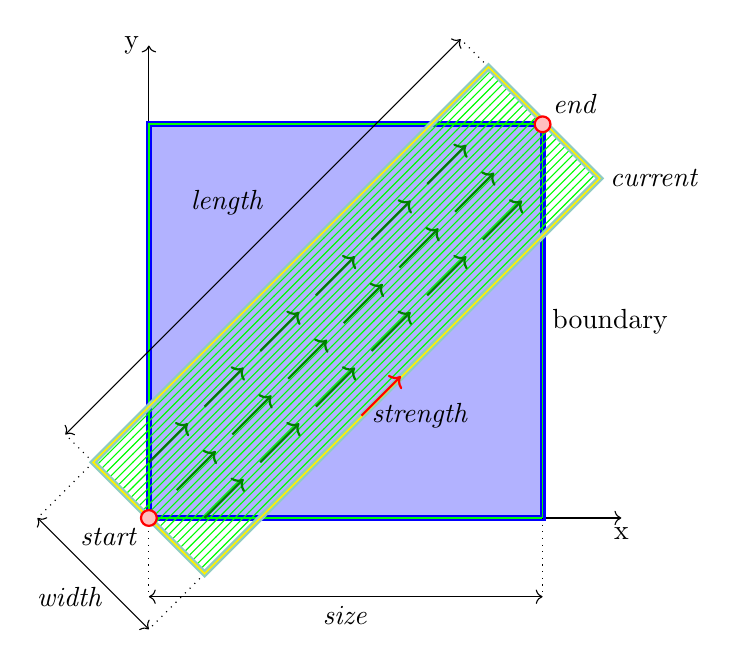
\begin{tikzpicture}

\draw[<->] (0,6) node[left] {y} -- (0,0) -- (6,0) node[below] {x};

\draw[thick, double, double=green, blue, fill=blue!30!white] (0,0)rectangle(5,5);
\draw (5,2.5) node[right] {boundary};
\draw[dotted] (0,0) -- (0,-1);
\draw[<->] (0,-1) -- (5,-1);
\draw[dotted] (5,0) -- (5,-1);
\draw (2.5,-1) node[below] {\emph{size}};

\draw[rotate=-45, xshift=-0.5cm, <->] (-1,0) -- (-1,7.1);
\draw[rotate=-45, dotted] (-1,0) -- (-1.5,0);
\draw[rotate=-45, dotted] (-1,7.1) -- (-1.5,7.1);
\draw (1,4) node {\emph{length}};

\draw[rotate=-45, yshift=-1cm, <->] (-1,0) -- (1,0);
\draw[rotate=-45, dotted] (-1,0) -- (-1,-1);
\draw[rotate=-45, dotted] (1,0) -- (1,-1);
\draw (-1,-1) node {\emph{width}};

\draw[rotate=-45, thick, double, double=yellow, color=green!30!white!80!blue, pattern color=green ,pattern=north east lines] (-1,0)rectangle(1,7.1) node[black, right] {\emph{current}};

\draw[->, red, thick, xshift=0.7cm, yshift=-0.7cm] (2,2) node[right, black] {\emph{strength}} -- (2.5,2.5);

\draw[thick, color=red, fill=pink] (0,0) node[anchor=north east, black] {\emph{start}} circle (0.1);
\draw[thick, color=red, fill=pink] (5,5) node[anchor=south west, black] {\emph{end}} circle (0.1);


\foreach \x/\angle in {-0.5/90, 0/90, 0.5/90} {
    \foreach \y in {0.5, 1.5, 2.5, 3.5, 4.5, 5.5} {
        \draw[->,thick, rotate=-45, green!50!black]  (\x, \y) -- ++(\angle:0.7);
    }
}

\end{tikzpicture}

% 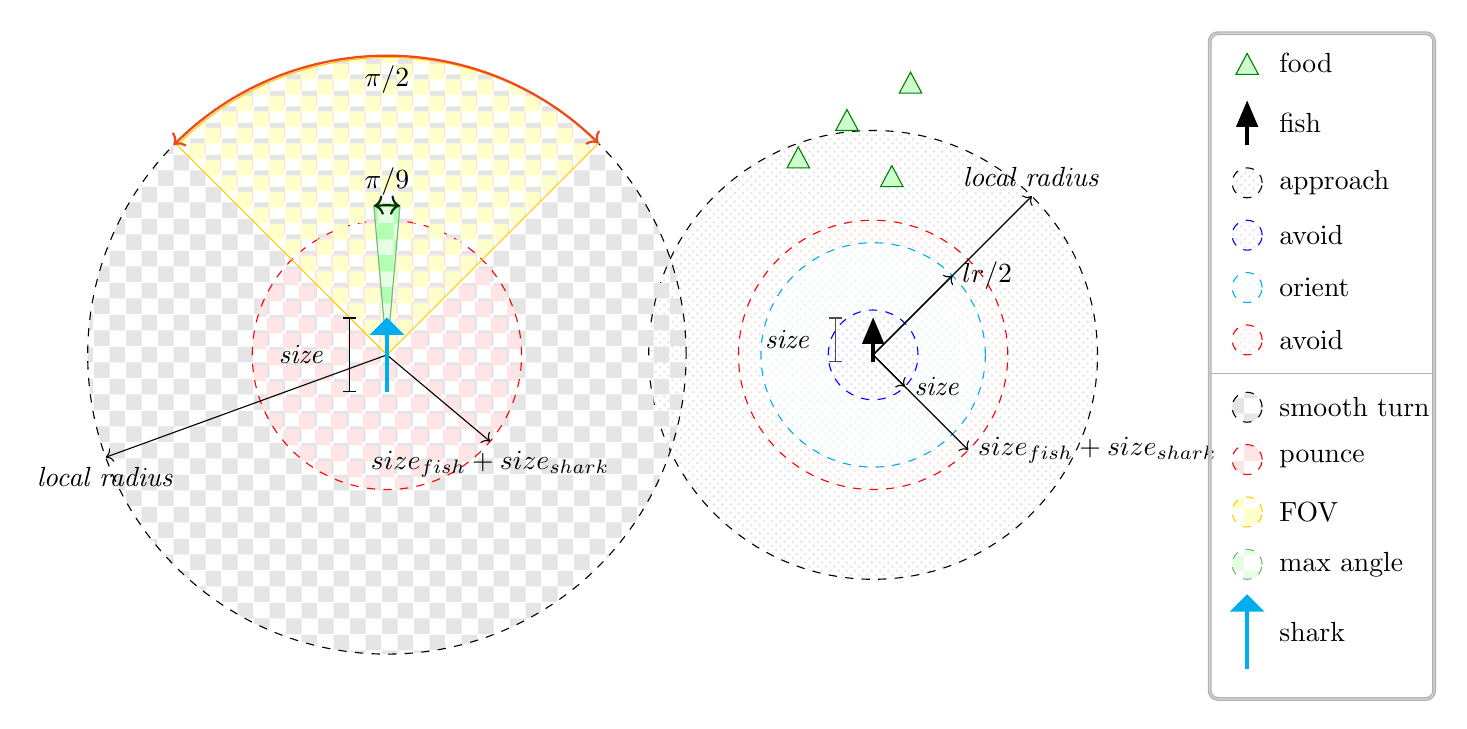
\begin{tikzpicture}[scale=0.95]

\draw[dashed, pattern=crosshatch dots, pattern color=black!10] (0,0)circle(3);
\draw[dashed, color=red, pattern=crosshatch dots, pattern color=red!10] (0,0)circle(1.8);
\draw[dashed, color=cyan, pattern=crosshatch dots, pattern color=cyan!10] (0,0)circle(1.5);
\draw[dashed, color=blue, pattern=crosshatch dots, pattern color=blue!10] (0,0)circle(0.6);

\filldraw[green!50!black, fill=green!20, yshift=-0.5cm, xshift=0.5cm] (-0.15,4) -- (0.15,4) -- (0,4.28) -- cycle;
\filldraw[green!50!black, fill=green!20, yshift=-1cm, xshift=-0.35cm] (-0.15,4) -- (0.15,4) -- (0,4.28) -- cycle;
\filldraw[green!50!black, fill=green!20, yshift=-1.5cm, xshift=-1cm] (-0.15,4) -- (0.15,4) -- (0,4.28) -- cycle;
\filldraw[green!50!black, fill=green!20, yshift=-1.75cm, xshift=0.25cm] (-0.15,4) -- (0.15,4) -- (0,4.28) -- cycle;

\draw[thin, ->] (0,0) -- (45:3);
\draw[thin, ->] (0,0) -- (45:1.5);
\draw[thin, ->] (0,0) -- (-45:1.8);
\draw[thin, ->] (0,0) -- (-45:0.6);
\draw (45:3) node[above] {\textit{local radius}};
\draw (45:1.5) node[right] {$lr/ 2$};
\draw (-45:1.8) node[right] {$size_{fish} + size_{shark}$};
\draw (-45:0.6) node[right] {\textit{size}};

\draw[very thick, -triangle 45] (0,-0.1) -- (0,0.5);
\draw[|-|, black!70!] (-0.5,-0.1) -- (-0.5,0.5);
\draw (-0.7,0.2) node[left] {\textit{size}};

\draw[dashed, pattern=crosshatch dots, pattern color=black!10, xshift=10.5cm, yshift=1.3cm] (-5.5,1)circle(0.2);
\draw[xshift=10.5cm, yshift=1.3cm] (-5.2,1) node[right] {approach};
\draw[dashed, color=blue, pattern=crosshatch dots, pattern color=blue!10, xshift=10.5cm, yshift=1.3cm] (-5.5,0.3)circle(0.2);
\draw[xshift=10.5cm, yshift=1.3cm] (-5.2,0.3) node[right] {avoid};
\draw[dashed, color=cyan, pattern=crosshatch dots, pattern color=cyan!10, xshift=10.5cm, yshift=1.3cm] (-5.5,-0.4)circle(0.2);
\draw[xshift=10.5cm, yshift=1.3cm] (-5.2,-0.4) node[right] {orient};
\draw[dashed, color=red, pattern=crosshatch dots, pattern color=red!10, xshift=10.5cm, yshift=1.3cm] (-5.5,-1.1)circle(0.2);
\draw[xshift=10.5cm, yshift=1.3cm] (-5.2,-1.1) node[right] {avoid};

\draw[xshift=10.5cm, yshift=1.3cm, black!30] (-6,-1.55) -- (-3,-1.55);

\draw[dashed, pattern=checkerboard, pattern color=black!10, xshift=10.5cm, yshift=1.1cm] (-5.5,-1.8)circle(0.2);
\draw[xshift=10.5cm, yshift=1.1cm] (-5.2,-1.8) node[right] {smooth turn};
\draw[dashed, color=red, pattern=checkerboard, pattern color=red!10, xshift=10.5cm, yshift=1.1cm] (-5.5,-2.5)circle(0.2);
\draw[xshift=10.5cm, yshift=1.1cm] (-5.2,-2.5) node[right] {pounce};
\draw[dashed, color=red!20!yellow, pattern=checkerboard, pattern color=yellow!20, xshift=10.5cm, yshift=1.1cm] (-5.5,-3.2)circle(0.2);
\draw[xshift=10.5cm, yshift=1.1cm] (-5.2,-3.2) node[right] {FOV};
\draw[dashed, color=green!40!black!50, pattern=checkerboard, pattern color=green!10, xshift=10.5cm, yshift=1.1cm] 
(-5.5,-3.9)circle(0.2);
\draw[xshift=10.5cm, yshift=1.1cm] (-5.2,-3.9) node[right] {max angle};

\draw[xshift=10.5cm, yshift=1.3cm, very thick, -triangle 45] (-5.5,1.5) -- (-5.5,2.1);
\draw[xshift=10.5cm, yshift=1.3cm] (-5.2,1.8) node[right] {fish};

\filldraw[green!50!black, fill=green!20, xshift=10.5cm, yshift=1.3cm] (-5.65,2.45) -- (-5.35,2.45) -- (-5.5,2.73) -- cycle;
\draw[xshift=10.5cm, yshift=1.3cm] (-5.2,2.6) node[right] {food};

\draw[xshift=10.5cm, yshift=1.1cm, very thick, -triangle 90, cyan] (-5.5,-5.3) -- (-5.5,-4.3);
\draw[xshift=10.5cm, yshift=1.1cm] (-5.2,-4.8) node[right] {shark};

\draw[black!30!, double, double=black!20, rounded corners=3pt, xshift=10.5cm, yshift=1.3cm] (-6,3)rectangle(-3,-5.9);

\filldraw[dashed, pattern=checkerboard, pattern color=black!10, xshift=-6.5cm] (0,0)circle(4);

\draw[dashed, color=red, pattern=checkerboard, pattern color=red!10, xshift=-6.5cm] (0,0)circle(1.8);

\filldraw[red!20!yellow, pattern=checkerboard, pattern color=yellow!20, xshift=-6.5cm] (0,0) -- (45:4) arc (45.5:135:4) -- cycle;
\draw[<->, xshift=-6.5cm, yellow!20!red, thick] (45:4) arc (45:135.5:4);
\draw[xshift=-6.5cm] (0,4) node[below] {$\pi/2$};

\filldraw[green!30, xshift=-6.5cm] (0,0) -- (85:2) arc (85:95:2) -- cycle;
\filldraw[green!40!black!50, pattern=checkerboard, pattern color=green!10, xshift=-6.5cm] (0,0) -- (85:2) arc (85:95:2) -- cycle;
\draw[<->, xshift=-6.5cm, green!20!black, thick] (85:2) arc (85:95:2);
\draw[xshift=-6.5cm] (0,2) node[above] {$\pi/9$};

\draw[thin, ->, xshift=-6.5cm] (0,0) -- (200:4);
\draw[xshift=-6.5cm] (200:4) node[below] {\textit{local radius}};
\draw[thin, ->, xshift=-6.5cm] (0,0) -- (-40:1.8);
\draw[xshift=-6.5cm] (-40:1.8) node[below] {$size_{fish} + size_{shark}$};
%\draw[xshift=-6.5cm] (0,4) node[above] {\textit{field of view}};

\draw[very thick, -triangle 90, cyan, xshift=-6.5cm] (0,-0.5) -- (0,0.5);
\draw[|-|, xshift=-6.5cm] (-0.5,-0.5) -- (-0.5,0.5);
\draw[xshift=-6.5cm] (-0.7,0.0) node[left] {\textit{size}};


\end{tikzpicture}

% 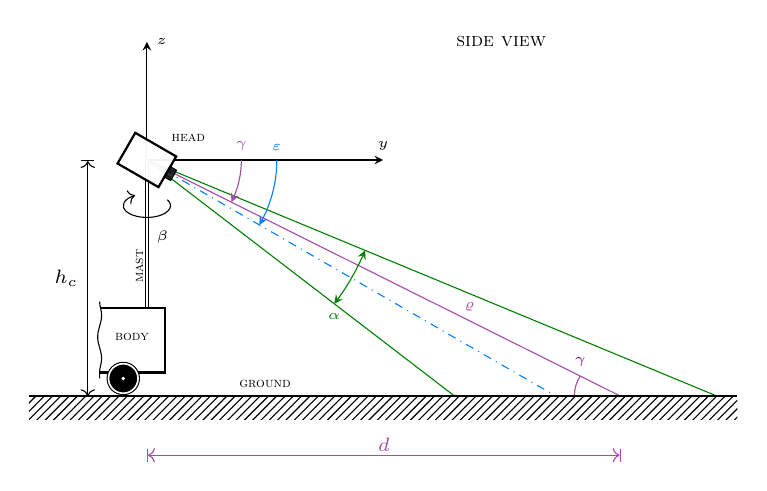
\begin{tikzpicture}[scale=1.5]
\tikzset{translate/.style={shift={(#1)}}}
\tikzstyle{ground} = [fill, pattern=north east lines, draw=none, minimum width=0.75cm, minimum height=0.3cm]

\draw[stealth-stealth] (0,3) node[right] {\tiny{$z$}} -- (0,2) -- (2,2) node[above] {\tiny{$y$}};

\draw[violet!70, thin] (0,2) -- +(-30+3.5:4.482317);
\draw[violet!70, thin] ([translate=-30+3.5:4.1]0,2) node[above, violet] {\tiny{$\gamma$}} arc (146.5:180:0.3);

\node[violet!70] at ([translate=-30+5.5:3]0,2) {\tiny{$\varrho$}};

\draw[|<->|, violet!70] (0,-0.5) -- (4.011379417,-0.5);
\node[violet!70, above] at (2.005689708,-0.55) {\scriptsize{$d$}};

\draw[dashdotted, blue!50!cyan] (0,2) -- +(-30:4);

\draw[thin, green!50!black] (0,2) -- +(-37.5:3.2854);
\draw[thin, green!50!black] (0,2) -- +(-30+7.5:5.226252);

\draw[double] (0,0.75) -- (0,2);

\draw[thick] (-0.4,0.75) -- (0.15,0.75) -- (0.15,0.2) -- (-0.4,0.2);
\draw[decorate, decoration={snake, segment length=5.5mm, amplitude=0.25mm}] (-0.4,0.8) -- (-0.4,0.15);
\draw[fill=black, double] (-0.2,0.15) circle (0.125);
\draw[fill=white, white] (-0.2,0.15) circle (0.01);
\node at (-0.125,0.5) {\tiny{\textsc{body}}};

\draw[rotate around={-30:(0,2)}, fill=white, fill opacity = 0.95, thick] (-0.2,1.85) rectangle (0.2,2.15);

\draw[rotate around={-30:(0,2)}, fill=black, fill opacity = 0.8, xshift=6] (-0.015,1.95) rectangle (0.05,2.05);
\node[above] at (0.35,2.075) {\tiny{\textsc{head}}};

\draw[-stealth, violet!70] (0.8,2) node[above] {\tiny{$\gamma$}} arc (0:-30+3.5:0.8);
\draw[-stealth, blue!50!cyan] (1.1,2) node[above] {\tiny{$\varepsilon$}} arc (0:-30:1.1);

\node[above, rotate=90] at (0.05,1.1) {\tiny{\textsc{mast}}};

\draw[<->|] (-0.5,0) -- (-0.5,2);
\node[left] at (-0.5,1) {\scriptsize{$h_c$}};

\draw[green!50!black, stealth-stealth] ([translate=-30+7.5:2]0,2) arc (-30+7.5:-37.5:2) node[below] {\tiny{$\alpha$}};

\draw[ground] (-1,0) rectangle (5,-0.2);
\draw[thick] (-1,0) -- (5,0);

\draw[<-] (-0.1,1.7) arc (120:390:0.2 and 0.1);
\node[right] at (0,1.35) {\tiny{$\beta$}};

\node at (1,0.1) {\tiny{\textsc{ground}}};

\node at (3,3) {\scriptsize{\textsc{side view}}};

\end{tikzpicture}

\tdplotsetmaincoords{60}{120}

\begin{tikzpicture}[scale=2.75,tdplot_main_coords]

\draw[pattern=north east lines, draw=none, opacity=0.5] (0,-0.1,-0.1) -- (0,0.5,-0.1) -- (0,0.5,0.26) -- (0,-0.1,0.26) -- cycle;

\filldraw[white] (0,0,0.16) -- (0,0.42,0.16) -- (0,0.42,0) -- (3.9,0.42,0) -- (3.9,0,0) -- (3.9,0,0.16) -- cycle;
\filldraw[white!50!cyan, opacity=0.3] (0,0,0.095) -- (0,0.42,0.095) -- (0,0.42,0) -- (3.9,0.42,0) -- (3.9,0,0) -- (3.9,0,0.095) -- cycle;
%\filldraw[white!50!red, opacity=0.3] (0,0,0.16) -- (0,0.42,0.16) -- (0,0.42,0.095) -- (3.9,0.42,0.095) -- (3.9,0,0.095) -- (3.9,0,0.16) -- cycle;
\filldraw[white!30!yellow!90!red, opacity=0.3] (0,0,0.16) -- (0,0.42,0.16) -- (0,0.42,0.095) -- (3.9,0.42,0.095) -- (3.9,0,0.095) -- (3.9,0,0.16) -- cycle;


\draw[black!30, dashed] (3.9,0,0) -- (0,0,0) -- (0,0,0.095) -- (0,0,0.16);
\draw[black!30, dashed] (0,0,0) -- (0,0.42,0);
\draw[black!30, dashed] (3.9,0,0.095) -- (0,0,0.095) -- (0,0,0.095) -- (0,0.42,0.095);
\draw[] (0,0.42,0.095) -- (3.9,0.42,0.095) -- (3.9,0,0.095);
\draw[] (0,0,0.16) -- (0,0.42,0.16) -- (0,0.42,0) -- (3.9,0.42,0) -- (3.9,0,0) -- (3.9,0,0.16) -- cycle;
\draw[] (0,0.42,0.16) -- (3.9,0.42,0.16) -- (3.9,0,0.16);
\draw[] (3.9,0.42,0) -- (3.9,0.42,0.16);

\draw[black!50, ultra thin] (3.9,0,0) -- (3.9,0,-0.1);
\draw[black!50, ultra thin] (3.9,0.42,0) -- (3.9,0.42,-0.1);
\draw[<->, ultra thin] (3.9,0,-0.1) -- (3.9,0.42,-0.1);
\node[below, black!50] at (3.9,0.21,-0.1) {\tiny{b}};

\draw[<->, ultra thin] (3.9,0.42,-0.1) -- (0,0.42,-0.1);
\draw[black!50, ultra thin] (0,0.42,0) -- (0,0.42,-0.1);
\node[below, black!50] at (1.8,0.42,-0.1) {\tiny{L}};

\draw[<->, ultra thin] (3.9,-0.05,0) -- (3.9,-0.05,0.095);
\draw[ultra thin, black!50] (3.9,0,0) -- (3.9,-0.05,0);
\draw[ultra thin, black!50] (3.9,0,0.095) -- (3.9,-0.05,0.095);
\node[left, black!50] at (3.9,-0.05,0.04525) {\tiny{$h_2$}};

\draw[<->, ultra thin] (3.9,-0.05,0.095) -- (3.9,-0.05,0.16);
\draw[ultra thin, black!50] (3.9,0,0.16) -- (3.9,-0.05,0.16);
\node[left, black!50] at (3.9,-0.05,0.16) {\tiny{$h_1$}};

%draw the main coordinate system axes
\draw[-stealth, green!50!black!60] (0,0,0) -- (0.3,0,0) node[anchor=north]{\tiny{$y$}};
\draw[-stealth, green!50!black!60] (0,0,0) -- (0,0.2,0) node[anchor=north]{\tiny{$x$}};
\draw[-stealth, green!50!black!60] (0,0,0) -- (0,0,0.25) node[anchor=south]{\tiny{$z$}};

\tdplotsetmaincoords{0}{0}
\begin{scope}[scale=0.5,tdplot_main_coords, xshift=-3.5cm]
\draw[ultra thin, black!50] (-0.7,0.2) rectangle (0.96,-1.45);
\node[text width=2cm] at (0.3,0) {\tiny{$L=3.9\,mm$}};
\node[text width=2cm] at (0.3,-0.25) {\tiny{$b=0.42\,mm$}};
\node[text width=2cm] at (0.3,-0.5) {\tiny{$h_1=0.065\,mm$}};
\node[text width=2cm] at (0.3,-0.75) {\tiny{$h_2=0.095\,mm$}};
\draw (-0.5,-0.95) rectangle (-0.4,-1.05);
%\draw[fill=white!50!red, opacity=0.3] (-0.5,-0.95) rectangle (-0.4,-1.05);
\draw[fill=white!30!yellow!90!red, opacity=0.3] (-0.5,-0.95) rectangle (-0.4,-1.05);
\node[text width=2cm] at (0.5,-1) {\tiny{piezo-ceramic}};
\draw (-0.5,-1.2) rectangle (-0.4,-1.3);
\draw[fill=white!50!cyan, opacity=0.3] (-0.5,-1.2) rectangle (-0.4,-1.3);
\node[text width=2cm] at (0.5,-1.25) {\tiny{steel}};

\node at (2.8,0.3) {\tiny{\textsc{root}}};
\node at (-0.5,-2.7) {\tiny{\textsc{tip}}};

\draw[ultra thin] (3,0.27) -- (3.8,0.15);
\draw[ultra thin] (-0.45,-2.8) -- (0,-3.15);
\end{scope}

\end{tikzpicture}


\end{document}